In this chapter we shall explore ways in which we can infer the topological properties of topological dynamical systems by using topological and symbolic relationships. In Section \ref{sec:topological-conjugacy} we shall introduce topological conjugacy, a term used to describe when two maps exhibit the same topological behaviour. This section will include proving that various topological properties hold through topological conjugacy and introduce examples of topologically conjugate system. In Section \ref{sec:symbolic-dynamics} we shall develop symbolic methods of characterising topological dynamical systems using infinite sequences of symbols. This proves useful for describing the topological dynamics of various topological dynamical systems where the dynamics are easier to explain using sequences of symbols. As a result this section will allow us to prove compelling results about the tent and doubling maps. Section \ref{sec:sharkovskys-theorem-and-type} will then introduce the reader to Sharkovsky's theorem, a very important result which explains when that if a topological dynamical system  defined over intervals on $\mathbb{R}$ has a period three point, then it has points of all other periods. Furthermore we shall then show how we can contruct topological dynamical systems over closed intervals with a specific set of periods as defined by Sharkovsky's order.

\section{Topological Conjugacy} \label{sec:topological-conjugacy}
As mentioned above, topological conjugacy defines when two maps exhibit the same topological behaviour and can be considered equivalent. If two maps are topologically conjugate, properties we have proved for one map can be applied to the other. Hence topological conjugacy is a powerful relationship when studying the dynamics of related topological dynamical systems. Note that just as in Section \ref{sec:topological-dynamical-systems}, the definitions below apply generally to continuous maps, however have been formulated in terms of topological dynamical systems for clarity and precisison. First, lets introduce our main definition.

\begin{defn}[Topological Conjugacy] \label{defn:topological-conjugacy}
    Let $(X, f)$ and $(Y, g)$ be topological dynamical systems. The topological dynamical system $(Y, g)$ is \emph{topologically semi-conjugate} to $(X, f)$ if there exists a continuous, surjective map $\varphi: X \to Y$ termed a \emph{topological conjugacy} where $\varphi \circ f = g \circ \varphi$. Furthermore if $\varphi$ is a homeomorphism i.e. $\varphi$ is a bijection with $\varphi$ and $\varphi^{-1}$ both continuous then $(Y, g)$ is \emph{topologically conjugate} to $(X, f)$. In this case $\varphi$ is called a \emph{topological conjugacy}.
\end{defn}

\begin{center}
\begin{tikzpicture}
    \node(lt) {$X$};
    \node(rt) [right=of lt] {$X$};
    \node(lb) [below=of lt] {$Y$};
    \node(rb) [below=of rt] {$Y$};

    \draw[->] (lt.east) -- node[above] {$f$} (rt.west);
    \draw[->] (lb.east) -- node[above] {$g$} (rb.west);
    \draw[->] (lt.south) -- node[left] {$\varphi$} (lb.north);
    \draw[->] (rt.south) -- node[right] {$\varphi$} (rb.north);
\end{tikzpicture}
\end{center}

The diagram above is a termed commutative diagram and shows the relationship between the topological dynamical systems and the topological conjugacy. If $\varphi$ is a topological semi-conjugacy then this diagram commutes. If $\varphi$ is a just semi-conjugacy the topological dynamics of $(X, f)$ are carried over to $(Y, g)$, however if since $\varphi$ is not a homeomorphism the reverse does not hold generally. Only when $\varphi$ is homeomorphic and so a topological conjugacy do the dynamics of $(Y, g)$ carry over into $(X, f)$. Now we shall prove that the topological dynamical systems $T_2$ and $F_4$ are topologically conjugate and that $T_2$ and $D$ are topologically semi-conjugate. We shall see later in Section \ref{sec:symbolic-dynamics} that they also share the same topological dynamics.

\begin{prop} \label{prop:tent-logistic-conjugate}
    The tent map $([0, 1], T_2)$ and the logistic map $([0, 1], F_4)$ are topologically conjugate.
    \begin{proof}
        Let $\varphi: [0, 1] \to [0,1]$ be defined by $\varphi(x) = \sin^2(\frac{\pi x}{2})$ which is homeomorphic on $[0, 1]$ as is continuous, bijective and $\varphi^{-1} = \frac{2}{\pi} \sin^{-1}(\sqrt{x})$ exists and is continuous on $[0, 1]$. Clearly we have, \[F_4 \circ \varphi(x) = 4 \sin^2\left(\frac{\pi x}{2}\right) \cdot \left(1 - \sin^2\left(\frac{\pi x}{2}\right)\right) = 4 \sin^2\left(\frac{\pi x}{2}\right) \cos^2\left(\frac{\pi x}{2}\right) = \sin^2\pi x, \ \text{for} \ x \in [0, 1]\] \[\varphi \circ T_2(x) = \varphi(2x) = \sin^2\pi x, \ \text{for} \ x \in \left[0, 1/2\right]\] \[\varphi \circ T_2(x) = \varphi(2(1 - x)) = \sin^2 (\pi (1-x)) = \sin^2 \pi x, \ \text{for} \ x \in [1/2, 1]\] Hence we have shown that $\varphi \circ T_2 = F_4 \circ \varphi$ so $F_4$ and $T_2$ are topologically conjugate.
    \end{proof}
\end{prop}

\begin{prop} \label{prop:tent-doubling-semi-conjugate}
    The tent map $([0, 1], T_2)$ and the doubling map $([0, 1], D)$ are topologically semi-conjugate.
    \begin{proof}
        Let $\varphi: [0, 1] \to [0, 1]$ be the tent map $T_2$ which is continuous and surjective. From the definition $\varphi(x) = 2x$ if $x \in \left[0, \frac{1}{2}\right]$ and $\varphi(x) = 2(1-x)$ if $x \in \left[\frac{1}{2}, 1\right]$. Then separating by cases we have, \[\varphi \circ D(x) = 2(2x) = 4x \ \text{and} \ T_2 \circ \varphi(x) = 2(2x) = 4x, \ \text{if} \ x \in \left[0, 1/4\right]\] \[\varphi \circ D(x) = 2(1 - (2x)) = 2 - 4x \ \text{and} \ T_2 \circ \varphi(x) = 2(1-2x) = 2 - 4x, \ \text{if} \ x \in \left[1/4, 1/2\right]\] \[\varphi \circ D(x) = 2(2x-1) = 4x - 2 \ \text{and} \ T_2 \circ \varphi(x) = 2(1-2(1-x)) = 4x - 2, \ \text{if} \ x \in \left[1/2, 3/4\right]\] \[\varphi \circ D(x) = 2(1-(2x - 1)) = - 4x + 4 \ \text{and} \ T_2 \circ \varphi(x) = 2(2(1-x)) = -4x + 4, \ \text{if} \ x \in \left[3/4, 1\right]\] Hence $\varphi \circ D = T_2 \circ \varphi$, so $D$ and $T_2$ are topologically semi-conjugate.
    \end{proof}
\end{prop}

Topological conjugacy preserves topological dynamical properties. For instance if topological dynamical systems $(X, f)$ and $(Y, g)$ are topologically conjugate through some map $\varphi$ then if $x$ is a fixed point of $f$, $\varphi(x)$ is a fixed point of $g$. This can be proved as $\varphi(x) = \varphi \circ f(x) = g \circ \varphi(x)$. This next lemma will prove the more general result for period-$k$ points.

\begin{prop} \label{prop:conjugacy-preserves-periodic-points}
    Let $(X, f)$ and $(Y, g)$ be topological dynamical systems and let $\varphi: X \to Y$ be a topological semi-conjugacy. If $x$ is a period-$k$ point of $f$ then $\varphi(x)$ is a period-$k$ point of $g$. Furthemore if $\varphi$ is a topological conjugacy then if $\varphi(x)$ is a period-$k$ point of $g$ then $x$ is a period-$k$ point of $f.$
    \begin{proof}
        Suppose $f^k(x) = x$, then by induction $\varphi(x) = \varphi \circ f^k(x) = g^k \circ \varphi (x)$. Since $\varphi$ is invertible $f^k(x) = \varphi \circ f^k \circ \varphi^{-1}(x)$. Now suppose $g^k(\varphi(x)) = \varphi(x)$, then $x = \varphi \circ \varphi^{-1}(x) = g^k \circ \varphi \circ \varphi(x)^{-1} = \varphi \circ f^k \circ \varphi^{-1}(x) = f^k(x)$.
    \end{proof}
\end{prop}

Therefore, to understand the periodic points of one dynamical system we can analyse the the periodic points of another system which is topologically conjugate to it. This becomes useful when dealing with dynamical sytems which have particularly complex behaviour. This next proposition states that topological conjugacy holds for iterations of the maps $f^n$ and $g^n$.

\begin{prop} \label{prop:conjugacy-preserved-under-iterations}
    Let $(X, f)$ and $(Y, g)$ be topological dynamical systems and $n \in \mathbb{N}$. If $\varphi: X \to Y$ is a topological semi-conjugacy from $(X, f)$ to $(Y, g)$ then $\varphi$ is a topological semi-conjugacy from $(X, f^n)$ to $(X, g^n)$
    \begin{proof}
        Let $\varphi$ be a topological semi-conjugacy, so $\varphi \circ f = g \circ \varphi$. Hence, $\varphi \circ f^n = \varphi \circ f \circ f^{n-1} = g \circ \varphi \circ f \circ f^{n-2} = \dots = g^{n-1} \circ \varphi \circ f = g^n \circ \varphi$.
    \end{proof}
\end{prop}

Further topological properties that conjugacy preserves are the following.

\begin{prop} \label{prop:conjugacy-preserves-orbits}
    Let $(X, f)$ and $(Y, g)$ be topological dynamical systems and let $\varphi: X \to Y$ be a topological semi-conjugacy with $x \in X$. If $\mathcal{O}_f(x)$ is an orbit of $f$ then $\mathcal{O}_g(\varphi(x))$ is an orbit of $g$.
    \begin{proof}
        Let $x \in X$ with $y = \varphi(x)$. By definition, $\mathcal{O}_f(x) = \left\lbrace f^n(x) : n \geq 0 \right\rbrace$. Hence applying $\varphi$ to the orbit we obtain $\varphi\left(\mathcal{O}_f(x)\right) = \left\lbrace \varphi \circ f^n(x) : n \geq 0 \right\rbrace = \left\lbrace g^n \circ \varphi(x) : n \geq 0 \right\rbrace = \mathcal{O}_g(\varphi(x))$ using Proposition \ref{prop:conjugacy-preserved-under-iterations}.
    \end{proof}
\end{prop}

Stated alternatively, topological conjugacy ensures orbits in $(X, f)$ are sent to orbits in $(Y, g)$. This next proposition follows directly from the proposition above.

\begin{prop} \label{prop:conjugacy-preserves-dense-orbits}
    Let $(X, f)$ and $(Y, g)$ be topological dynamical systems and let $\varphi: X \to Y$ be a topological semi-conjugacy. If $f$ has a dense orbit in $X$ then $g$ has a dense orbit in $Y$.
    \begin{proof}
        Before we begin, note that, from topology, if $f: X \to Y$ is a continuous, surjective function and $\overline{E} = X$ then $\overline{f(E)} = Y$. Now suppose $x \in X$ has a dense orbit in $f$, so $\overline{\mathcal{O}_f(x)} = X$. By definition, $\varphi$ is continuous and surjective, hence $\overline{\varphi(\mathcal{O}_{f}(x))} = \overline{\mathcal{O}_{g}(\varphi(x))} = Y$ by Proposition \ref{prop:conjugacy-preserves-orbits}. Hence $g$ has a dense orbit in $Y$.
    \end{proof}
\end{prop}

\begin{prop} \label{prop:conjugacy-preserves-dense-periodic-points}
    Let $(X, f)$ and $(Y,g)$ be topological dynamical systems and let $\varphi: X \to Y$ be a topological semi-conjugacy. If $Per(f)$ are dense in $X$ then $Per(g)$ are dense in $Y$.
    \begin{proof}
        Suppose $\overline{Per(f)} = X$. By continuity, $g(Y) \circ \varphi = \varphi \circ f(X) = \varphi \circ f(\overline{Per(f)}) \subseteq \varphi \circ \overline{f(Per(f))} = \overline{g(Per(g))} \circ \varphi$. Hence $g(Y) \subseteq \overline{g(Per(g))}$. Hence $Per(g)$ is dense in $Y$.
    \end{proof}
\end{prop}

Proposition's \ref{prop:conjugacy-preserves-dense-orbits} and \ref{prop:conjugacy-preserves-dense-periodic-points} turns out to be important in proving examples of topological dynamical systems are chaotic. Concluding this section, note the wide range of topological dynamics that is preserved between topologically conjugate systems. We shall apply these results in the next section on symbolic dynamics as we further characterise complex topological dynamics.

\section{Symbolic Dynamics} \label{sec:symbolic-dynamics}
Symbolic dynamics studies how the shift map effects infinite sequences of symbols, called itineries, that describe the complex dynamics of specific topological dynamical systems. More specifically it is the assignment of a sequence of discrete symbols to the orbits of topological dynamical systems. This proves useful as in specific instances, like the tent map and doubling map over the unit interval, the behaviour of topological dynamical systems becomes easier to characterise using topologically conjugate, topological dynamical systems described symbolically using itineries. In the process of applying symbolic dynamics to a topological dynamical system we separate the underlying metric space into finitely many labeled partitions. We then generate a so called itinerary by noting the infinite sequence of symbols obtained, describing the inclusion of a point in a partition for successive iterations of the map. This sequence is an element in the so called sequence space; and it is in this space where we can study the discrete dynamics of the topological system. Lets now define this notion concretely.

\begin{defn}[Itinerary] \label{defn:itinerary}
    Let $(X, f)$ be a topological dynamical system where $X$ is a compact set. Let $x \in X$ and suppose $X = X_0 \cup X_1 \cup \dots \cup X_n$ where $X_i$ are compact sets. The \emph{itinerary} of $x$ is the sequence $\underline{s} = (s_1s_2\dots)$ where $s_i$ denotes the set $X_i$ such that $f^i(x) \in X_i$.
\end{defn}

\begin{figure}[h]
    \centering
    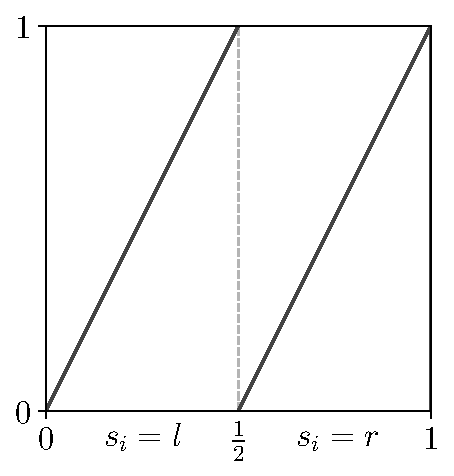
\includegraphics[width=4cm]{doubling_symbolic}
    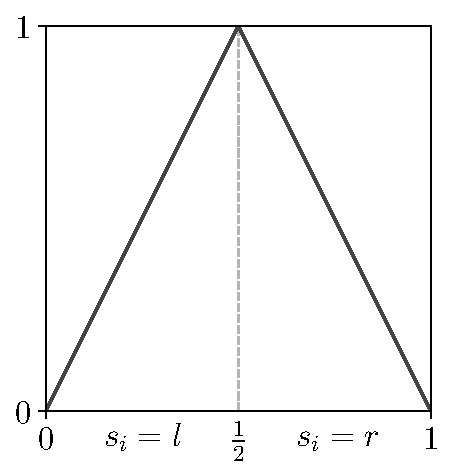
\includegraphics[width=4cm]{tent_symbolic}
    \caption{Itineraries for the tent map $([0, 1], T_2)$ and the doubling map $([0, 1], D)$ respectively.}
    \label{fig:symbolic}
\end{figure}

Figure \ref{fig:symbolic} gives an example of useful itineraries for the tent map and doubling map. Properties of the itinerary reflect properties of the topological dynamical system it represents. If a point the topological dynamical system is periodic, then that same point will give a periodic itinerary. Now we shall construct a metric space in which where the underlying set contains all possible itineries of zeros and ones.

\begin{defn}[Sequence Space] \label{defn:sequence-space}
    Let $\Sigma_2 = \left\lbrace (s_1s_2\dots): s_i \in \left\lbrace 0, 1 \right\rbrace \right\rbrace$ be the set of itineraries of zeros and ones. Define $(\Sigma_2, d)$ to be the \emph{sequence space} where $d(s, t) = \Sigma_{i=1}^{\infty}|s_i - t_i|2^{-i}$ is a metric for $(s)_{i=1}^{\infty} = (s_1s_2\dots) \in \Sigma_2$ and $(t)_{i=1}^{\infty} = (t_1t_2\dots) \in \Sigma_2$. It can be easily shown this is a metric space.
\end{defn}

A useful map to have symbol dynamics would be one that maps each point in a compact set to its itinerary in sequence space. Hence we have the following definition.

\begin{defn}[Itinerary Map] \label{defn:itinerary-map}
    Let $X$ be a compact set and $\Sigma_2$ be the sequence space. Suppose $x \in X$. Define $\pi : X \to \Sigma_2$ to be the \emph{itinerary map} where $\pi(x) = (s_1s_2\dots)$ i.e.\ $\pi$ maps each $x \in X$ to its itinerary.
\end{defn}

A property that we want the sequence space to have is for it to be compact. Hence we can then use it a the underlying metric space for some topological dynamical systems. Therefore, we shall now prove in the following proposition that it is compact.

\begin{prop}
    The sequence space $(\Sigma_2, d)$ where $d(s, t) = \Sigma_{i=1}^{\infty}|s_i - t_i|2^{-i}$ is compact.
    \begin{proof}
        Let $(x_n)_n$ be a Cauchy sequence in $\Sigma_2$. Let $k \in \mathbb{N}$, where $x_i(k)$ denotes the $k$-th element of $x_i$. The sequence $x_1(k),x_2(k)\dots$ is eventually constant as if not we can find $n, m \in \mathbb{N}$ such that $x_n(N) \neq x_m(N)$ for some $N \in \mathbb{N}$ and hence $d(x_n, x_m) \geq \frac{1}{2^N}$, a contradiction. Let $s_k$ be the eventually constant term in $(x_n)_n$. Hence we can construct $s = ( s_k : k \in \mathbb{N} ) \in \Sigma_2$ such that the sequence $(x_n)_n$ converges to $s$. We have proved $\Sigma_2$ is complete. Let $\varepsilon > 0$ and choose $N$ such that $\frac{1}{2^{N - 1}} \leq \varepsilon$. Hence $\left\lbrace B_d(s, \varepsilon) : s \in \Sigma_2 \ \text{where} \ s_k = 0, \ \forall\, k \geq N\right\rbrace$ cover $\Sigma_2$. Hence $\Sigma_2$ is totally bounded and so is compact.
    \end{proof}
\end{prop}

Now that we have proved $(\Sigma_2, d)$ is a compact metric space, if we have an associated continuous mapping $f: \Sigma_2 \to \Sigma_2$ then we have a topological dynamical system. Hence we can now introduce an important topological dynamical system to the study of symoblic dynamics.

\begin{defn} [Shift Map]
    Let $(s)_{i=1}^{\infty} \in \Sigma_2$. The \emph{shift map} $\sigma: \Sigma_2 \to \Sigma_2$ is given by $\sigma \left((s)_{i=1}^{\infty}\right) = (s)_{i=2}^{\infty}$ and describes a topological system $(\Sigma_2, \sigma)$.
\end{defn}

Thereby, the shift map removes the first element from a sequence. We shall now prove that the shift map is continuous and so $(\Sigma_2, \sigma)$ is a topological dynamical system.

\begin{prop}
    The shift map $\sigma: \Sigma_2 \to \Sigma_2$ is continuous.
    \begin{proof}
        Let $\varepsilon > 0$ and suppose $\underline{s} = (s_i)_{i=1}^{\infty}, \ \underline{t} = (t_i)_{i=1}^{\infty} \in \Sigma_2$. Choose $\delta = \varepsilon$ and suppose $d(\underline{s}, \underline{t}) = \Sigma_{i=1}^{\infty}|s_i - t_i|2^{-i} < \delta$. Then $d\left( \sigma\left(\underline{s}\right) - \sigma\left(\underline{t}\right) \right) = d\left((s)_{i=2}^{\infty} - (t)_{i=2}^{\infty}\right) = \Sigma_{i=2}^{\infty}|s_i - t_i|2^{-i} \leq \Sigma_{i=1}^{\infty}|s_i - t_i|2^{-i} < \delta = \varepsilon$.
    \end{proof}
\end{prop}

Since $(\Sigma_2, \sigma)$ defines a topological dynamical system we shall use symbolic dynamics to prove a few important properties about it, which will come in useful when characterising chaos in Chapter \ref{chap:defining-chaos}. For now remember these results, from \cite[\S 1.6]{devaney}, as we will be referring back to them.

\begin{prop} \label{prop:shift-map-periodic-points-dense}
    The periodic points of the shift map $(\Sigma_2, \sigma)$ are dense in $\Sigma_2$.
    \begin{proof}
        Let $\underline{s} = (s)_{i=1}^{\infty}$ be an arbitrary point in $\Sigma_2$. Define $t_n = (s_0\dots s_ns_0\dots s_n\dots)$ to be an infinite repeating sequence where $t_{n_i} = s_i$ for $1 \leq i \leq n$. Then $d(s, t) = \sum_{i = 0}^n|s_i - s_i|2^{-i} + \sum_{i=n+1}^{\infty}|s_i - t_i|2^{-i} \leq \sum_{i = n+1}^{\infty}2^{-i} = 2^{-n}$. Hence as $n \to \infty$ we have $t_n \to \underline{s}$. Since $\underline{s}$ was arbitrary, the periodic points of $\sigma$ are dense.
    \end{proof}
\end{prop}

\begin{prop} \label{prop:shift-map-dense-orbit}
    The shift map $(\Sigma_2, \sigma)$ has a dense orbit.
    \begin{proof}
        Consider the sequence $\underline{s} = (0\ 1\ |\ 00\ 01\ 10\ 11\ |\ 000\ 001\ \dots\ |\ \dots)$ contructed by writing down all possible combinations of blocks of length one to infinity. Let $\underline{t} = (t)_{i=0}^{\infty} \in \Sigma_2$ be arbitrary. Let $\varepsilon > 0$. By construction we can perform some $k$ number of iterations of $\sigma$ such that if $n > N + k = \frac{1}{\varepsilon} + k$ iterations of $\sigma$ such that $d(\underline{s}, \underline{t}) = \sum_{i = k}^{n}|s_i - t_i|2^{-i} + \sum_{i = n+1}^{\infty}|s_i - t_i|2^{-i} \leq \sum_{i = n+1}^{\infty}|s_i - t_i|2^{-i} = 2^{-n} < 2^{-N} < \frac{1}{N} = \varepsilon$. Hence the orbit $\underline{s}$ is dense in $\Sigma_2$.
    \end{proof}
\end{prop}

Symbolic dynamics has an elegant application to various maps such as the tent map and doubling map. We shall first investigate the doubling map, then we can later apply these results to the tent map. The nature of the doubling map $D: [0, 1] \to [0, 1]$ makes binary expansions a suitable choice for expressing points in this map. For each $x \in [0, 1]$ we can write $x=\sum_{i=1}^{\infty}b_i2^{-i}$ where $b_i \in \left\lbrace 0, 1 \right\rbrace$. This next propostion describes an important relationship between the doubling map and the shift map which we shall expolore through the use of binary expansions.

\begin{prop} \label{prop:doubling-shift-semi-conjugate}
    The doubling map $([0, 1], D)$ and the shift map $(\Sigma_2, \sigma)$ are semi-conjugate via the semi-conjugacy $\varphi: \Sigma_2 \to [0, 1]$.
    \begin{proof}
        Let $\underline{b} = (b_i)_{i=1}^{\infty} \in \Sigma_2$ be a sequence of binary digits and let $\underline{c} = \sigma\left((b_i)_{i=1}^{\infty}\right) = (c_i)_{i=1}^{\infty} \in \Sigma_2$ where $c_i = b_{i + 1}$ be the sequence $\underline{b}$ shifted once. Define the map $\varphi: \Sigma_2 \to [0, 1]$ where $\varphi\left((b_i)_{i=1}^{\infty}\right) = \sum_{i=1}^{\infty} b_i2^{-i} \in [0, 1]$. Let $\sigma: \Sigma_2 \to \Sigma_2$ be the shift map. The function $\varphi$ is surjective, as every point $x \in [0, 1]$ has at least one binary expansion denoted $x=\sum_{i=1}^{\infty}b_i2^{-i}$ where $b_i \in \left\lbrace 0, 1 \right\rbrace$.
        \begin{center}
            \begin{tikzpicture}
                \node(lt) {$\Sigma_2$};
                \node(rt) [right=of lt] {$\Sigma_2$};
                \node(lb) [below=of lt] {$[0, 1]$};
                \node(rb) [below=of rt] {$[0, 1]$};
            
                \draw[->] (lt.east) -- node[above] {$\sigma$} (rt.west);
                \draw[->] (lb.east) -- node[above] {$D$} (rb.west);
                \draw[->] (lt.south) -- node[left] {$\varphi$} (lb.north);
                \draw[->] (rt.south) -- node[right] {$\varphi$} (rb.north);
            \end{tikzpicture}
        \end{center}
        Using an arbitrary $\underline{b} \in \Sigma_2$, $\varphi \circ \sigma\left((b_i)_{i=1}^{\infty}\right) = \varphi\left((c_i)_{i=1}^{\infty}\right) = \sum_{i=1}^{\infty} c_i2^{-i} = \sum_{i=1}^{\infty} b_{i+1}2^{-i} \in [0, 1]$. Similarly $D \circ \varphi\left((b_i)_{i=1}^{\infty}\right) = D\left(\sum_{i=1}^{\infty} b_i2^{-i}\right) = \sum_{i=1}^{\infty} 2b_i2^{-i} \mmod 1 = b_1 + \sum_{i=2}^{\infty} b_i2^{-i+1} \mmod 1 = \sum_{i=2}^{\infty} b_i2^{-i+1} = \sum_{j=1}^{\infty} b_{j+1}2^{-j} \in [0, 1]$. Hence we have shown $\varphi \circ \sigma = D \circ \varphi$. and so the doubling map $D$ and the shift map $\sigma$ are semi-conjugate via $\varphi$. We can also see $\varphi$ is not injective as $\frac{1}{2} + \sum_{i=2}^{\infty}0 \cdot 2^{-i} = \sum_{i=2}^{\infty}2^{-i} = \frac{1}{2}$ and so $\varphi$ is not a homeomorphism and hence is simply a semi-conjugacy. 
    \end{proof}
\end{prop}

Intuitively this makes sense as the doubling map acts as a shift on the binary expansion of a number. Moreover, the semi-conjugacy $\varphi$ can be thought of as an inverse itenerary map as defined in Definition \ref{defn:itinerary-map}. We can use this semi-conjugacy gained via symbolic dynamics to now prove that the periodic points in the doubling map $D$ and by extension the logistic map $F_4$ and the tent map $T_2$ are dense.

\begin{prop} \label{prop:logisitc-tent-doubling-periodic-dense}
    The periodic points of the logistic map $([0, 1], F_4)$, the tent map $([0, 1], T_2)$ and the doubling map $([0, 1], D)$ are dense in $[0, 1]$.
    \begin{proof}
    By Proposition \ref{prop:tent-logistic-conjugate} the logistic map $([0, 1], F_4)$ is conjugate to the tent map $([0, 1], T_2)$. Similarly, by Proposition \ref{prop:tent-doubling-semi-conjugate} the tent map $([0, 1], T_2)$ is semi-conjugate to the doubling map $([0, 1], D)$. By Proposition \ref{prop:doubling-shift-semi-conjugate} the doubling map $([0, 1], D)$ is semi-conjugate to the shift map $(\Sigma_2, \sigma)$. In Proposition \ref{prop:shift-map-periodic-points-dense} the shift map $\sigma$ has periodic orbits. Finally by Proposition \ref{prop:conjugacy-preserves-dense-orbits} dense orbits are preserved under semi-conjugacy so $D, \ T_2$ and $F_4$ all have periodic points that are dense in $[0, 1]$.
    \end{proof}
\end{prop}

\begin{center}
    \begin{tikzpicture}
        \node(l1) {$\Sigma_2$};
        \node(r1) [right=of l1] {$\Sigma_2$};
        \node(l2) [below=of l1] {$[0, 1]$};
        \node(r2) [below=of r1] {$[0, 1]$};
        \node(l3) [below=of l2] {$[0, 1]$};
        \node(r3) [below=of r2] {$[0, 1]$};
        \node(l4) [below=of l3] {$[0, 1]$};
        \node(r4) [below=of r3] {$[0, 1]$};
    
        \draw[->] (l1.east) -- node[above] {$\sigma$} (r1.west);
        \draw[->] (l2.east) -- node[above] {$D$} (r2.west);
        \draw[->] (l1.south) -- node[left] {$\varphi_1$} (l2.north);
        \draw[->] (r1.south) -- node[right] {$\varphi_1$} (r2.north);

        \draw[->] (l3.east) -- node[above] {$T_2$} (r3.west);
        \draw[->] (l2.south) -- node[left] {$\varphi_2$} (l3.north);
        \draw[->] (r2.south) -- node[right] {$\varphi_2$} (r3.north);

        \draw[->] (l4.east) -- node[above] {$F_4$} (r4.west);
        \draw[->] (l3.south) -- node[left] {$\varphi_3$} (l4.north);
        \draw[->] (r3.south) -- node[right] {$\varphi_3$} (r4.north);
    \end{tikzpicture}
\end{center}

The power of topological conjugacy and symbolic dynamics is clear from Proposition \ref{prop:logisitc-tent-doubling-periodic-dense}. It shows how we can use symbolic dynamics to build properties about a simple topological dynamical system like the shift map, then use topological conjugacy to show that these properties hold for more complex dynamical systems. Proposition \ref{prop:logisitc-tent-doubling-periodic-dense} will be extremely useful when generating examples of chaotic topological dynamical systems in Chapter \ref{chap:defining-chaos}.

\section{Sharkovsky's Theorem and Type}\label{sec:sharkovskys-theorem-and-type}
Sharkovsky's forcing theorem, often abbriviated to Sharkovsky's theorem \cite{sharkovsky}, is a consequential theorem in the study of topological dynamics. The theorem only applies to topological dynamical systems defined over closed intervals, however is still a powerful result. It states that if such a topological dynamical system has a period three point then periodic points of all other periods occur. Moreover the presense of a periodic point of given period implies the existence of other periods given by a total ordering called Sharkovsky's Order. Note that for the sake of brevity we shall note be proving Sharkovsky's theorem in this text. However, we shall prove a special case of Sharkovsky's theorem proved by Li and Yorke in their paper \emph{`Period Three Implies Chaos'} \cite{li-yorke} in which the existence of a period three point implies the existence of periodic points of all other periods. Note that as mentioned in the introduction this was the first paper that coined the term chaos in am matematical context. First, we will introduce a theorem that proves the existence of fixed points on closed intervals. This theorem is a simplified version of Brouwer's fixed-point theorem \cite{brouwer}. The full theorem is used to prove the existence of fixed points in a topological dynamical system where the underlying set is a subset of $\mathbb{R}^n$ and has the condition of being convex. Since Sharkovsky's theorem only requires the simplified theorem, we shall once again only prove this specialised case.

\begin{thm}[Brouwer's Fixed Point Theorem] \label{thm:interval-fixed-points}
    If $(I, f)$ is a topological dynamical system where $I$ is a closed interval and $I \subseteq f(I)$, then $f$ has a fixed point in $I$.
    \begin{proof}
        Let $I = [a, b]$ where $a, b \in \mathbb{R}$. Since $I \subseteq f(I)$ there exists $c, d \in I$ such that $f(c) = a$ and $f(d) = b$. Suppose $g(x) = f(x) - x$, then $g$ is continuous. Also $g(c) = a - c \geq 0$ and $g(d) = b - d \leq 0$. By the Intermediate Value Theorem there exists some $x \in I$ with $a \leq x \leq b$ such that $g(x) = 0$. Hence $f(x) = x$.
    \end{proof}
\end{thm}

Before we prove the theorem by Li and Yorke we shall explore intervals, coverings and loops through the following definition.

\begin{defn}[Covering, $N$-loop] \label{defn:covering}
    Let $J_0, J_1, \dots J_{n-1} \subseteq X$ be intervals and let $f: X \to X$ be a continuous map. The interval $J_0$ \emph{covers} $J_1$ if $J_1 \subseteq F(J_0)$ and is denoted $J_0 \xrightarrow{f} J_1$. A series of coverings $J_0 \xrightarrow{f} \cdots \xrightarrow{f} J_{n-1} \xrightarrow{f} J_0$ which starts and ends at the same interval is called a \emph{loop}, or specifically, \emph{n-loop} of intervals. A point $x \in X$ \emph{follows} the loop if $f^k(x) \in J_k$ for $0 \leq k \leq n-1$ and $f^n(x) = x$.
\end{defn}

Note that in this text, to denote a covering we will drop the $f$ and just write $J_0 \to J_1$ as we shall only deal with one map at a time and hence dont need to be explicit. The proof of \emph{`Period Three Implies Chaos'} \cite{li-yorke} relies upon us first deriving a set of intervals with specific coverings between them to form a loop. Once we have a loop we can then use Theorem \ref{thm:interval-fixed-points} to prove the existence of a periodic point with a period the size of this loop. This theorem is a specific case of Sharkovsky's theorem and hence is consise enough for us to prove in this text. The proof for this theorem follows work by Devaney \cite[\S 1.10]{devaney}.

\begin{thm}[Period Three Implies Chaos] \label{thm:period-three-chaos}
    Let $(I, f)$ be a topological dynamical system where $I$ is a closed interval. If $f$ has a point of period three, then $f$ has period points of all other periods.
    \begin{proof}
        Before we begin the proof note the following observation. If $A_0, A_1, \dots$ are closed intervals with $A_{i+1} \subseteq f(A_i)$ for $0 \leq i \leq n - 1$, i.e.\ $A_0 \to A_1 \cdots \to A_{n-1}$, then there exists a subinterval $J_0 \subseteq A_0$ such that $f(J_0) \subseteq A_1$. Similarly, there exists a subinterval $J_1 \subseteq A_1$ such that $f(J_1) \subseteq A_2$. Hence there exists a subinterval $J_1 \subseteq J_0$ such that $f(J_1) \subseteq A_1$ and $f^2(J_1) = A_2$. Continuing we get a nested sequence of intervals which are mapped in order into each $A_i$. Hence there exists some $x \in A_0$ such that $f^i(x) \in A_i$ for all $i$.
        \begin{figure}[H]
            \centering
            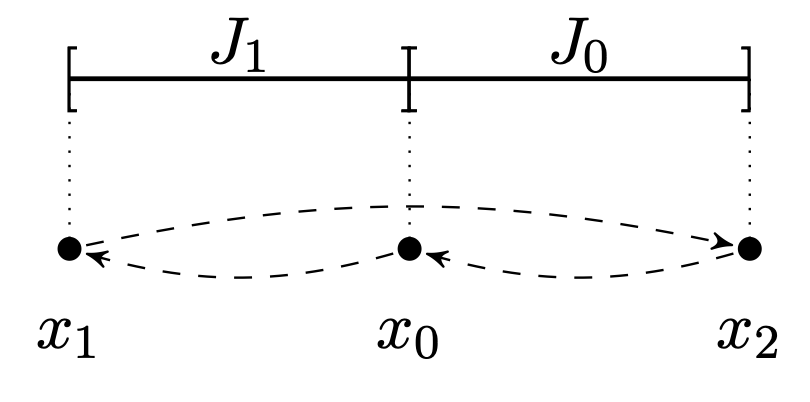
\includegraphics[width=4.5cm]{period3}
            \label{fig:periodthree}
        \end{figure}
        Now to begin the proof let $x_1, x_0, x_2 \in \mathbb{R}$ with $f(x_0) = x_1$, $f(x_1) = x_2$ and $f(x_2) = x_0$ and assume wlog that $x_1 < x_0 < x_2$. Let $J_1 = [x_1,x_0]$ and $J_0 = [x_0,x_2]$. Hence $J_1 \subseteq f(J_0)$ and $J_1 \cup J_0 \subseteq f(J_1)$. By Theorem \ref{thm:interval-fixed-points}, $f$ has a fixed point between $x_1$ and $x_0$. Similarly, $f^2$ has at least one fixed point between $x_0$ and $x_2$. Hence $f$ has a point of period 2. Now let $k \geq 2$. Define the nested sequence of intervals $A_0, A_1, \dots, A_{k-2} \subseteq J_1$ inductively. Let $A_0 = J_0$. Since $J_1 \subseteq f(J_1)$, there exists a subinterval $A_1 \subseteq A_0$ and $f(A_1) = A_0 = J_1$. Furthermore there exists a subinterval $A_2 \subseteq A_1$ such that $f(A_2) = A_1$ and therefore $f^2(A_2) = A_0 = J_1$. Continuing we get a subinterval $A_{k-2} \subseteq A_{k-3}$ such that $f(A_{k-2}) = A_{k-3}$. By the observation above if $x \in A_{k-2}$ then $f(x), f^2(x), \dots, f^{k-2}(x) \subseteq A_0$ so $f^{k-2}(A_{k-2}) = A_0 = J_1$. As $J_0 \subseteq f(J_1)$ there exists a subinterval $A_{k-1} \subseteq A_{k-2}$ such that $f^{k-1}(A_{k-1}) = J_0$. Since $J_1 \subseteq f(J_0)$, $J_1 \subseteq f^k(A_{k-1})$ so that $f^k(A_{k-1})$ covers $A_{k-1}$. Hence by our first observation $f^k$ has a fixed point $x$ in $A_{k-1}$ and so $f$ has a period-$k$ point in $A_{k-1}$. The first $k-2$ iterates of $x$ are in $J_1$, the $k-1$th iterate is in $J_0$ and the $k$th is $x$. If $f^{k-1}(x)$ is in the interior of $J_0$ then $x$ has period $k$. However, if $f^{k-1}(x)$ is in the boundary of $J_0$ then $k = 2$ or $3$.

        \begin{center}
            \begin{tikzpicture}[node distance=2.5cm]
                \node(lt) {$J_0$};
                \node(rt) [right=of lt] {$J_1$};
            
                \draw[->] ([yshift=3pt] lt.east) -- node[above] {$f^k(x) = x$} ([yshift=3pt] rt.west);
                \draw[->] ([yshift=-3pt] rt.west) -- node[below] {$f^{k-1}(x)$} ([yshift=-3pt] lt.east);
                \draw[->] (rt) to [out=410,in=310,loop,looseness=4.8] node[right] {$f^{i}(x)$ for $0 \leq i \leq k - 2$} (rt);
            \end{tikzpicture}
        \end{center}

    \end{proof}

\end{thm}
The diagram above demonstrates the behaviour. By Definition \ref{defn:covering} take $I_i \to I_j$ to mean that $f(J_i)$ covers $J_j$ i.e. $J_j \subseteq f(J_i)$. If $x \in J_1$ then we can produce a period-$k$ cycle for any $k \in \mathbb{N}$. This is because we can find a sequence of open intervals $J_1 \to A_1 \to \dots \to A_k \to J_1$ where $\left\lbrace A_i \in \left\lbrace J_1, J_0 \right\rbrace : 1 \leq i \leq k \right\rbrace$, and hence by Theorem \ref{thm:interval-fixed-points} find a fixed point for $f^k$ in $J_1$ and hence a period-$k$ point for $f$ in $J_1$. Hence as $J_1 \subset I$, $f$ has points of all other periods.

This consequences of this theorem are remarkable. If you can find a point of period three for a map $f$ then there exists periodic points of all other periods in the natural numbers; and hence periodic points exist with infinite periods. This theorem however does not show the bigger picture of whats going on here, for this we need to introduce Sharkovsky's theorem which is a full description of which periods imply the existence of other periods. However, before we get to the theorem, we require a total ordering termed Sharkovsky's order.

\begin{defn}[Sharkovsky's Order]
    The total ordering on the natural numbers, defined below, is named \emph{Sharkovsky's order}. \[ 3 \rhd 5 \rhd 7 \rhd 9 \rhd \dots \rhd 2 \cdot 3 \rhd 2 \cdot 5 \rhd \dots \rhd 2^2 \cdot 3 \rhd 2^2 \cdot 5 \rhd \dots \rhd \dots \rhd 2^3 \rhd 2^2 \rhd 2 \rhd 1 \]
\end{defn}

Hence the Sharkovsky ordering first enumerates all the odd integers multiplied by $2^k$ for $k \in \mathbb{N}$. This exhausts all the natural numbers apart from powers of two, which are then ordered last in descending order. Finally, this brings us to Sharkovsky's theorem.

\begin{thm}[Sharkovsky's Forcing Theorem] \label{thm:sharkovskys-forcing-theorem}
    Let $(I, f)$ be a topological dynamical system where $I$ is a closed interval. If $f$ has a period point of period $k$ then for all integers $l \lhd k$, $f$ has periodic points of period $l$.
\end{thm}

The proof of this theorem will be ommited since it is outwith the scope of this text, however can be found here \cite{sharkovsky}. Note however, that we proved the case where $k = 3$ and hence points with all other periods in Sharkovsky's order exist in Theorem \ref{thm:period-three-chaos}. Hence, it can be seen that this theorem more general that the one proved by by Li and Yorke \cite{li-yorke}, as period three is the greatest period in Sharkovsky's ordering hence its presense implies the existence of all other periods. Noticing the Sharkovsky ordering it can be seen that if there exists a periodic point in $f$ whose period is not a power of two, then $f$ has infinitely many many periodic points. The converse statement also holds. If $f$ has finitely many periodic points then they all must have periods that are powers of two. It can be useful to catagorise topological dynamical systems defined on a closed interval based on their periods. This leads us to the next definition from Ruette, \cite[\S 3.3]{ruette}.

\begin{defn}[Type] \label{def:type}
    Let $(I, f)$ be a topological dynamical system where $I$ is a closed interval and let $n \in \mathbb{N}$. Define the map $f$ to be of \emph{type} $n$ if the periods of periodic points of $f$ are the set $\left\lbrace m \in \mathbb{N} : m \unlhd n \right\rbrace$.
\end{defn}

Clearly every topological dynamical system over the closed intervals has a type. Sharkovsky also proved the converse, that there exists topological dynamical system over the closed intervals of every type in another important theorem termed Sharkovsky's Realisation Theorem. We shall state this theorem after the following example where we prove we can construct a type five topological dynamical system defined over the closed intervals.

\begin{exmp} \label{exmp:piecewise-sharkovsky}
    Let $([0, 4], f)$ be a piecewise linear map with $f(0) = 2$, $f(2) = 3$, $f(3) = 1$, $f(1) = 4$ and $f(4) = 0$. The map is displayed in Figure \ref{fig:piecewise_linear}. Clearly $f$ is continuous and $f$ has been constructed so that $0$ is a period-$5$ point. Moreover $f^3[0, 1] = [1, 4]$, $f^3[1, 2] = [2, 4]$ and $f^3[3, 4] = [0, 3]$, so $f^3$ has no fixed points in those intervals. However $f^3[2, 3] = [0, 4]$ hence by Theorem \ref{thm:interval-fixed-points}, $f^3$ has at least one fixed point in $[2, 3]$. Moreover $f: [2, 3] \to [1, 3]$, $f: [1, 3] \to [2, 5]$ and $f: [1, 4] \to [0, 4]$ are all monotonically decreasing on $[2, 3]$. Therefore $f^3$ is monotonically decreasing on $[2, 3]$ and so the fixed point is unique. Therefore this can only be the fixed point for $f$, and as such no period 3 point exists. Hence by Sharkovsky's forcing theorem, the map $f$ contains periodic points with the period of every natural number apart from 3. Therefore $f$ is of type $5$.

    \begin{figure}[h]
        \centering
        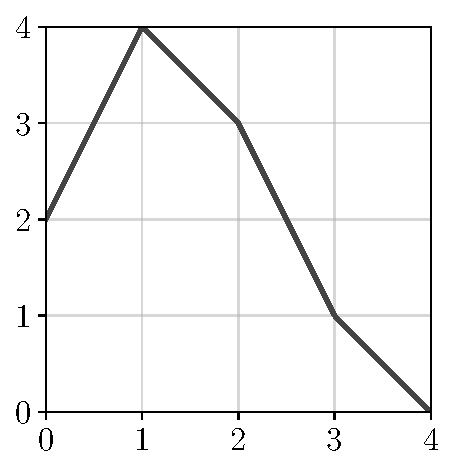
\includegraphics[width=4cm]{piecewise}
        \caption{Piecewise linear map $f$ with a period five point.}
        \label{fig:piecewise_linear}
    \end{figure}

\end{exmp}

Sharkovsky subsequently proved that topological dynamical systems over closed intervals can constructed to be of any type. In \cite{sharkovsky} he proves that you can construct maps with integer type, later in \cite{sharkovsky2} he proves you can construct maps with type in $2^\infty$. This theorem is termed Sharkovsky's Realisation Theorem and is stated below along with an elegant proof proved by Alseda, Llibre, and Misiurewicz \cite[\S 2.2]{alm} and outlined by Burns and Hasselblatt \cite[\S 7]{burns-hasselblatt}. This insightful proof uses properties of the trunctated tent map to reveal one number in the Sharkovsky ordering at a time.

\begin{thm}[Sharkovsky's Realisation Theorem] \label{thm:sharkovsky-realisation-theorem}
    Every tail of the Sharkovsky order is the set of periods for some map f in a topological dynamical system $(I, f)$ where $I$ is a closed interval.
    \begin{proof}
        Let $([0, 1], T_h)$ be a topological dynamical system, where $T_h(x) = \min(h, 1-2|x-1/2|)$ is the family of truncated tent maps with $h \in [0, 1]$, shown in Figure \ref{fig:truncated_tent}.
        \begin{figure}[h]
            \centering
            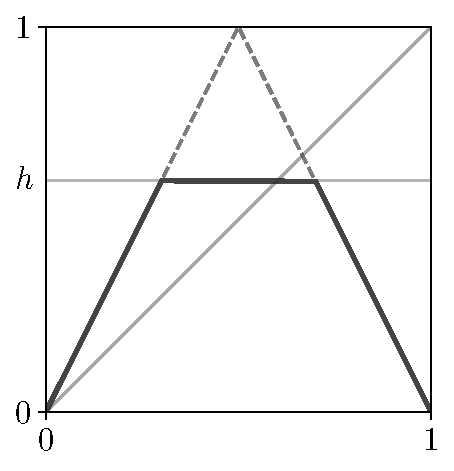
\includegraphics[width=4cm]{truncated_tent_2}
            \label{fig:truncated_tent}
            \caption{The truncated tent map $T_h$}
        \end{figure}
        It is clear that $T_0$ has only one periodic point, a fixed point at $x = 0$. However $T_1^3\left(\frac{2}{7}\right) = T_1^2\left(1-2\left\lvert\frac{2}{7} - \frac{1}{2}\right\rvert\right) = T_1^2\left(\frac{4}{7}\right) = T_1\left(1-2\left\lvert\frac{4}{7} - \frac{1}{2}\right\rvert\right) = T_1\left(\frac{6}{7}\right) = \left(1-2\left\lvert\frac{6}{7} - \frac{1}{2}\right\rvert\right) = \frac{2}{7}$. Hence $T_1$ has a period-$3$ point and so by Sharkovsky's Forcing Theorem has a periodic point for every period in the positive integers by Sharkovsky's Theorem. As $T_1$ and $T_h$ are identical on the interval $[0, h)$ any $k$-cycle $\mathcal{O}_{T_h}$ is also a $k$-cycle for $\mathcal{O}_{T_1}$ and any $k$-cycle $\mathcal{O}_{T_1}$ is also a $k$-cycle for $\mathcal{O}_{T_h}$. Now define the map $h: \mathbb{N} \to [0, 1]$ where $h(m) = \min \left\lbrace \max \mathcal{O}_{T_1} : \mathcal{O}_{T_1} \ \text{is $m$-cycle} \right\rbrace$, noting that $T_1^m$ has $2^m$ fixed points. Using the properties of the tent map we will find that the function $h$ we have constructed orders the natural numbers according to Sharkovskys ordering, with the set of periods of $T_h(m)$ being the tail of this ordering, starting from $m$. As the $k$-cycles for $\mathcal{O}_{T_h}$ and $\mathcal{O}_{T_1}$ are the same, $T_h$ has the $l$-cycle $\mathcal{O}_{T_h}$ if and only if $h(l) < h$. Moreover, $\mathcal{O}_{T_{h(m)}}$ is a $m$-cycle for $T_{h(m)}$, and all other cycles $\mathcal{O}_{T_{h(m)}}$ are contained within $[0, h(m))$. Using Sharkovsky's forcing theorem it is clear that if $m \rhd l$ then $T_{h(m)}$ has a period-$l$ orbit that lies in $[0, h(m))$ and hence $h(l) < h(m)$. Now by symmetry, $h(l) < h(m)$ if and only if $m \rhd l$. Hence we can see that for any positive integer $m$ the periodic points of $T_{h(m)}$ is the tail of the Sharkovsky order from $m \unrhd l$. Now for powers of two. By above $h(2^\infty) = \sup_k(h(2^k)) > h(2^k)$ for all $k \in \mathbb{N}$, so $T_{h(2^\infty)}$ has $2^k$-cycles for all $k \in \mathbb{N}$. Suppose $T_{h(2^\infty)}$ has an $m$-cycle with $m \neq 2^k$ for all $k \in \mathbb{N}$. Then by Sharkovsky's forcing theorem $T_{h(2^\infty)}$ has a $2m$-cycle. Because the $m$-cycle and $2m$-cycle are disjoint, at least one of them are contained in $[0, h(2^\infty))$ and hence in the interval $[0, h(2^k))$ for some $k \in \mathbb{N}$.
    \end{proof}
\end{thm}

Thus there exists a map $f$ and associated topological dynamical system $(I, f)$ such that $f$ has period-$k$ points and is of type $k$, where $k \in \mathbb{N}$ is in the Sharkovsky ordering. This concludes our study of Sharkovskys theorem and topological and symbolic relationships. In the next chapter on defining chaos we shall use the results we have developed here to prove that characteristics of chaos hold for certain topological dynamical systems.